% Appendix A

\chapter{Asynchronous Data Transfer Interface}

\label{AppendixA} % For referencing this appendix elsewhere, use \ref{AppendixA}

As shown in figure \ref{fig:AsyncInterface} the interface has three lines: 
value, ready, and acknowledge. The interface connects a Sender and Receiver.

\begin{figure}[H]
	\centering
	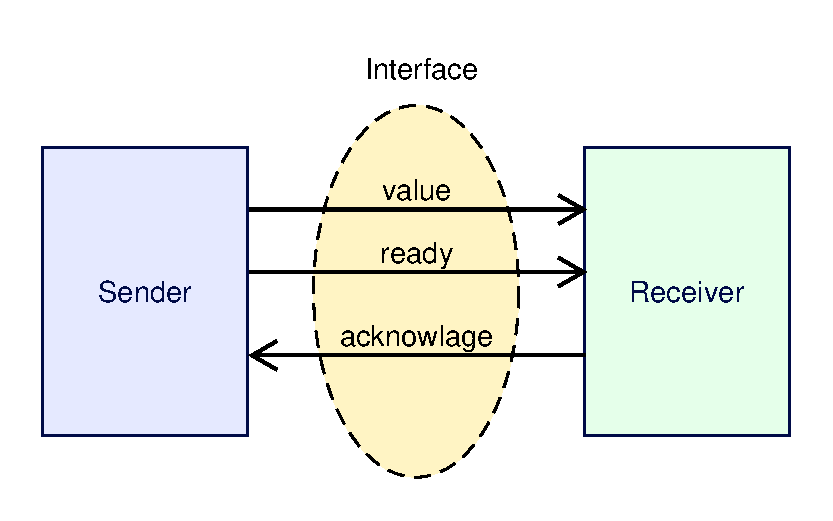
\includegraphics[scale=0.75]{Figures/AsyncInterface.pdf}
	\decoRule
	\caption{Asynchronous data transmission interface.}
	\label{fig:AsyncInterface}
\end{figure}

Data is sent on the \(value\) line, and the \(ready\) and \(acknowledge\) lines are
used for synchronization. The sender puts a value on the \(value\) line. The 
\(ready\) line is then switched. When the receiver has read the value the 
\(acknowledge\) line is switched.

\begin{figure}[H]
	\centering
	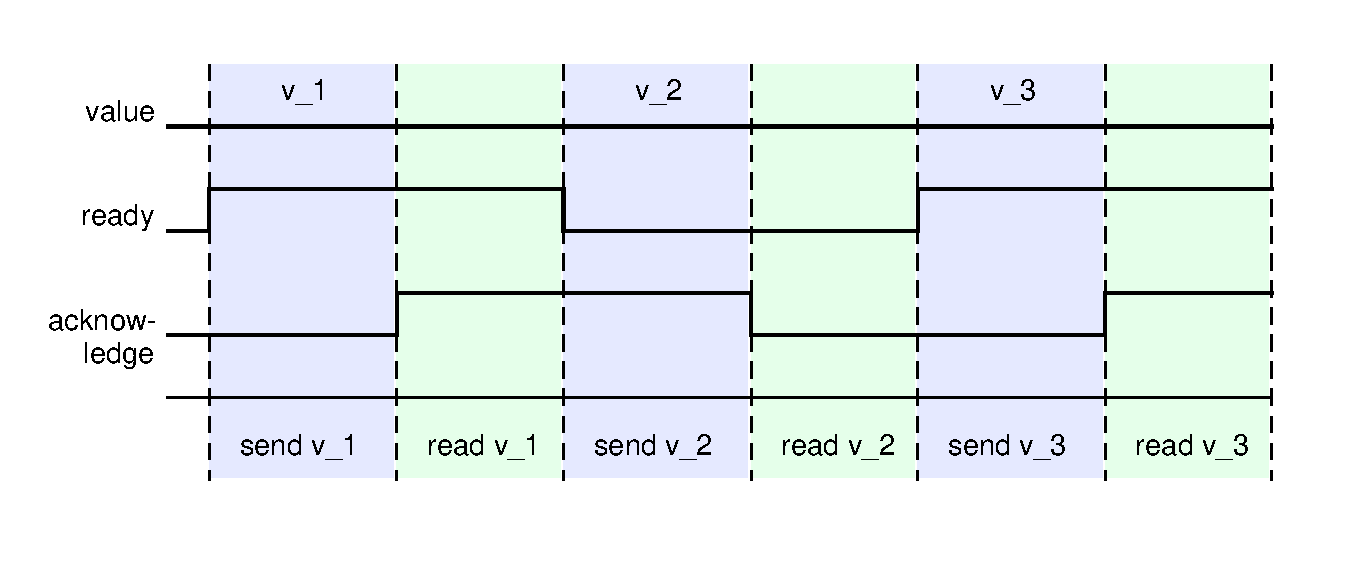
\includegraphics[scale=0.75]{Figures/AsyncInterface_send.pdf}
	\decoRule
	\caption{Asynchronous line transition states.}
	\label{fig:AsyncInterface_send}
\end{figure}